\let\negmedspace\undefined
\let\negthickspace\undefined
\documentclass[journal]{IEEEtran}
\usepackage[a5paper, margin=10mm, onecolumn]{geometry}
\usepackage{tfrupee} % Include tfrupee package

\setlength{\headheight}{1cm} % Set the height of the header box
\setlength{\headsep}{0mm}     % Set the distance between the header box and the top of the text

\usepackage{gvv-book}
\usepackage{gvv}
\usepackage{cite}
\usepackage{amsmath,amssymb,amsfonts,amsthm}
\usepackage{algorithmic}
\usepackage{graphicx}
\usepackage{textcomp}
\usepackage{xcolor}
\usepackage{txfonts}
\usepackage{listings}
\usepackage{enumitem}
\usepackage{mathtools}
\usepackage{gensymb}
\usepackage{comment}
\usepackage[breaklinks=true]{hyperref}
\usepackage{tkz-euclide} 
\usepackage{listings}
\def\inputGnumericTable{}                                 
\usepackage[latin1]{inputenc}                                
\usepackage{color}                                            
\usepackage{array}                                            
\usepackage{longtable}                                       
\usepackage{calc}                                             
\usepackage{multirow}                                         
\usepackage{hhline}                                           
\usepackage{ifthen}                                           
\usepackage{lscape}
\begin{document}

\bibliographystyle{IEEEtran}
\vspace{3cm}

\title{Matgeo-2.10.8}
\author{AI25BTECH11019 - MENAVATH SAI SANJANA}
{\let\newpage\relax\maketitle}

\renewcommand{\thefigure}{\theenumi}
\renewcommand{\thetable}{\theenumi}
\setlength{\intextsep}{10pt} % Space between text and floats

\numberwithin{equation}{enumi}
\numberwithin{figure}{enumi}
\renewcommand{\thetable}{\theenumi}

\textbf{Question}:\\
Let $\vec{b} = 4\hat{i} + 3\hat{j}$ and $\vec{c}$ be two vectors perpendicular to each other in the XY plane.  
All vectors in the same plane having projections $1$ and $2$ along $\vec{b}$ and $\vec{c}$, respectively, are given by .
\\
\bigskip

\textbf{Solution: } \\

Consider 
\begin{align}
\vec{r} = \myvec{r_1\\r_2},
\end{align}
where $r_1$ and $r_2$ are the x- and y-components of the required vector.

\begin{align}
\vec{b} &= \myvec{4\\3}, \quad
\vec{c} = \myvec{x\\y} \quad \text{(perpendicular to } \vec{b}\text{)}
\end{align}

\begin{align}
\text{Scalar projection on } \vec{b}: \quad 
\frac{\vec{r}^T \vec{b}}{\norm{\vec{b}}} = 1 
\quad \Rightarrow \quad \vec{r}^T \vec{b} = 5
\end{align}

\begin{align}
\text{Since } \vec{c} \perp \vec{b}, \quad 4x + 3y = 0 
\quad \Rightarrow \quad x = -3t,\; y = 4t
\end{align}

\begin{align}
\text{Scalar projection on } \vec{c}: \quad
\frac{\vec{r}^T \vec{c}}{\norm{\vec{c}}} = 2 
\quad \Rightarrow \quad \vec{r}^T \vec{c} = 10t
\end{align}

\begin{align}
\vec{r}^T \vec{b} &= 4 r_1 + 3 r_2 = 5 \\
\vec{r}^T \vec{c} &= -3 r_1 + 4 r_2 = 10
\end{align}

\begin{align}
\text{Solving:} \quad
r_1 &= -\frac{2}{5}, \quad r_2 = \frac{11}{5}
\end{align}

\bigskip
\noindent\textbf{Conclusion:}  
The required vector is
\begin{align}
\vec{r} = \myvec{-\tfrac{2}{5}\\ \tfrac{11}{5}}.
\end{align}

\begin{figure}[ht!]
    \centering
    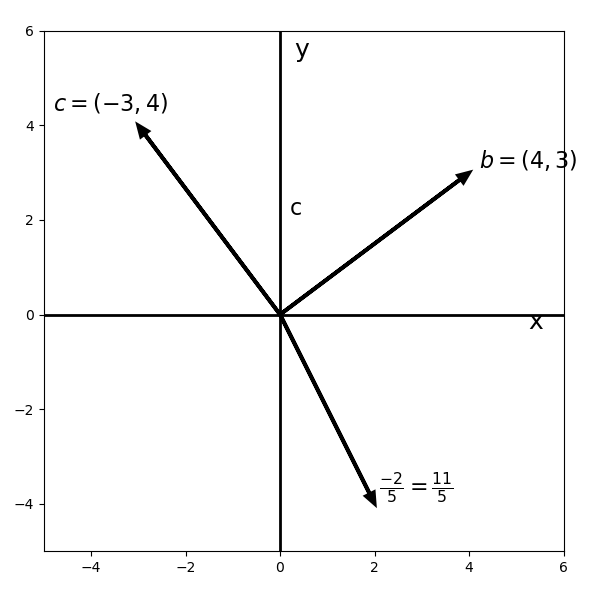
\includegraphics[width=0.9\textwidth]{figs/matgeo-2.10.8.png}
    \caption{}
    \label{fig:1.2.27.jpg}
\end{figure}

\end{document}

